We will now demonstrate the efficiency and robustness of Algorithm~\ref{Alg1}. \cref{fig:recon,fig:recon_msu} plot the reconstruction of two $256\times 256$ test images (shown in \cref{fig:true,fig:true_msu} respectively) from squared magnitude local measurements of the type described in \eqref{def:Measurements}.  Here $\a$ and $\b$ are chosen to be the {\em deterministic} measurement vectors of \cref{cor:2d_sparse} with $\delta$ chosen to be $2$.  The reconstructions were computed using an implementation of Algorithm~\ref{Alg1} in Matlab$^\circledR$ running on a Laptop computer (Ubuntu Linux 16.04 {\tt x86\_64}, Intel$^\circledR$ Core$^{\text{\tiny TM}}$M-5Y10c processor, 8GB RAM, Matlab$^\circledR$ R2016b).  More specifically, the linear measurement operator $\left. \mathcal M \right \vert_{\mathcal P}$ was constructed by passing the standard basis elements $E_{i,j}, i,j \in [d], |i-j|< \delta \mod d$ through \eqref{eq:2d_meas_op}.  An LU decomposition of this sparse and structured matrix was pre-computed and stored for different values of $d,\delta$ for use in the numerical simulations below.  We note that an FFT-based implementation of Step 1 of Algorithm~\ref{Alg1} is likely to yield improved efficiency; we defer such an implementation to future work.  The relative errors, defined by the expression $\displaystyle \frac{\min_\theta\Vert \mathbbm e^{\mathbbm i \theta} X-Q\Vert_F}{\Vert Q\Vert_F}$ (where $X$ denotes the reconstruction (up to a global phase factor) of $Q$), were $4.288\times 10^{-16}$ and $2.857\times 10^{-16}$ for the reconstructions in Figures \ref{fig:recon} and \ref{fig:recon_msu} respectively.  The reconstructions were computed in $16.318$ and $16.529$ seconds respectively.
%
\begin{figure}[p]
    \centering
    \begin{subfigure}[b]{0.495\textwidth}
        \centering
        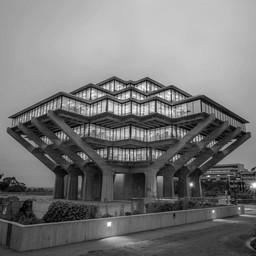
\includegraphics[scale=0.75]{2d_figs/true_ucsd}
        \caption{Test Image $1$ \\ ($256\times 256$ pixels)}
        \label{fig:true}
    \end{subfigure}
    \hfill
    \begin{subfigure}[b]{0.495\textwidth}
        \centering
        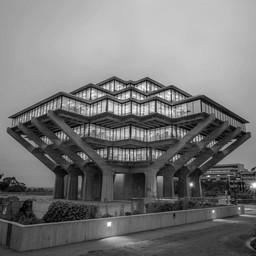
\includegraphics[scale=0.75]{2d_figs/recon_ucsd}
        \caption{Reconstructed Image (Rel. error $4.288\times 10^{-16}$)}
        \label{fig:recon}
    \end{subfigure}
    \vspace{0.05in} \\
    \begin{subfigure}[b]{0.495\textwidth}
        \centering
        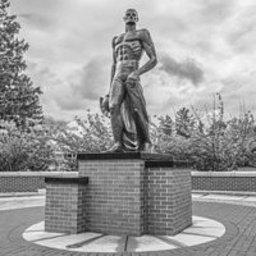
\includegraphics[scale=0.75]{2d_figs/true}
        \caption{Test Image $2$ \\ ($256\times 256$ pixels)}
        \label{fig:true_msu}
    \end{subfigure}
    \hfill
    \begin{subfigure}[b]{0.495\textwidth}
        \centering
        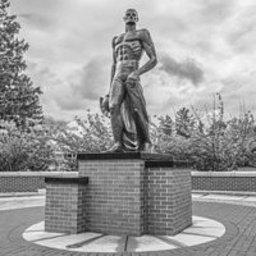
\includegraphics[scale=0.75]{2d_figs/recon}
        \caption{Reconstructed Image (Rel. error $2.857\times 10^{-16}$)}
        \label{fig:recon_msu}
    \end{subfigure}
    \vspace{0.05in}
    \caption{Two Dimensional Image Reconstruction from Phaseless Local Measurements.}
    \label{fig:2d-recon}
\end{figure}
%


We next plot the execution time (in seconds, averaged over $50$ trials) required to implement Algorithm~\ref{Alg1} for different values of $d$ in Fig. \ref{fig:etime}. In each case, $\delta$ was chosen to be $\lceil \log_2(d) \rceil$, with the same choice of measurement vectors as for the reconstruction in Fig.  \ref{fig:recon}. The plot confirms that the proposed method is extremely efficient; indeed, the plot reveals an FFT-time empirical computational complexity of $\mathcal O(d^2 \log_2(d^2))$.

Finally, Fig. \ref{fig:noise} illustrates the robustness of the proposed method to measurement errors.  The figure plots the reconstruction error (averaged over $50$ trials) in reconstructing a $64\times 64$ random matrix with i.i.d zero-mean complex Gaussian entries from phaseless measurements (with $\delta=6$, and with the same measurement construction as with Fig. \ref{fig:recon}). An additive noise model with i.i.d. zero-mean Gaussian noise was used to corrupt the measurements. The added noise as well as reconstruction error are reported in decibels,\footnote{Note that we distinguish $\SNRdb$ from $\SNR = \frac{\norm{\Ac(x x^*)}_2}{\norm{n}_2}$, though in the discussions of this section, we use ``SNR'' to refer to $\SNRdb$.}
%
\[  \SNRdb (dB) = 10 \log_{10}\left( \frac{\Vert \y \Vert_2^2}{d^2 D^2\sigma^2}\right), \qquad 
    \text{Error (dB)} = 10 \log_{10} \left( \frac{\min_\theta\Vert \mathbbm 
                e^{\mathbbm i \theta}X-Q\Vert^2_F}{\Vert Q\Vert^2_F}\right). \]
%
%For added robustness, an improved eigenvector-based magnitude estimation method detailed in 
%\cite[Section 6.1]{iwen2016phase} was utilized in place of Step 4 of Algorithm~\ref{Alg1}. 
%We observe that the proposed algorithm demonstrates robustness across a wide variety of SNRs. Moreover, 
%the test signals are reconstructed to (almost) the level of added noise. 
We observe that the proposed algorithm (indicated by the dashed line) demonstrates robustness across a wide variety of SNRs. Additionally, the results from utilizing an improved magnitude estimation method (detailed in \cref{sec:MagEstImpNumerical}) in place of Step 4 of Algorithm~\ref{Alg1} is plotted using the solid line. In both cases, we observe that the test signals are reconstructed to (almost) the level of added noise. 
%
\begin{figure}[hbtp]
    \centering
    \begin{subfigure}{0.495\textwidth}
        \centering
        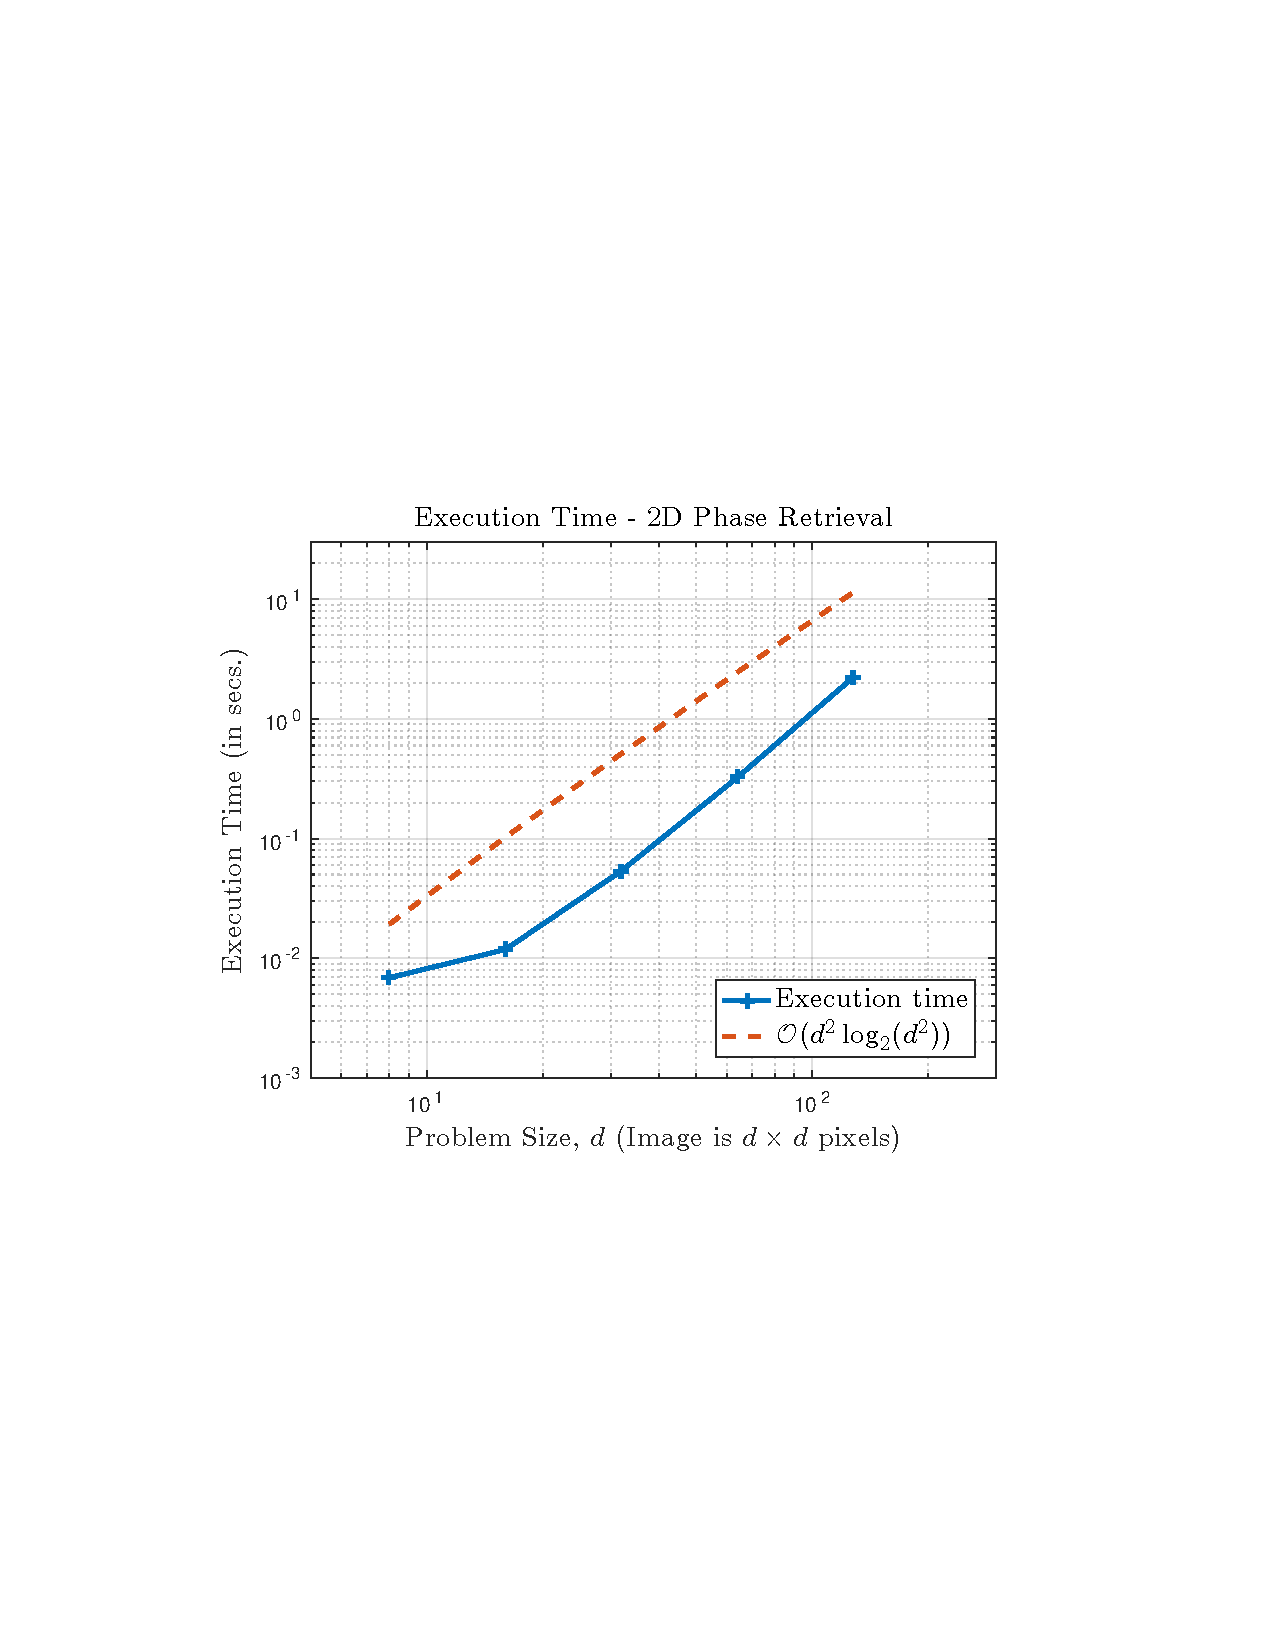
\includegraphics[clip=true, trim = 1.10in 3.25in 0.75in 3.25in,scale=0.55]{2d_figs/etime}
        \caption{Execution Time vs Problem Size}
        \label{fig:etime}
    \end{subfigure}
    \hfill
    \begin{subfigure}{0.495\textwidth}
        \centering
        %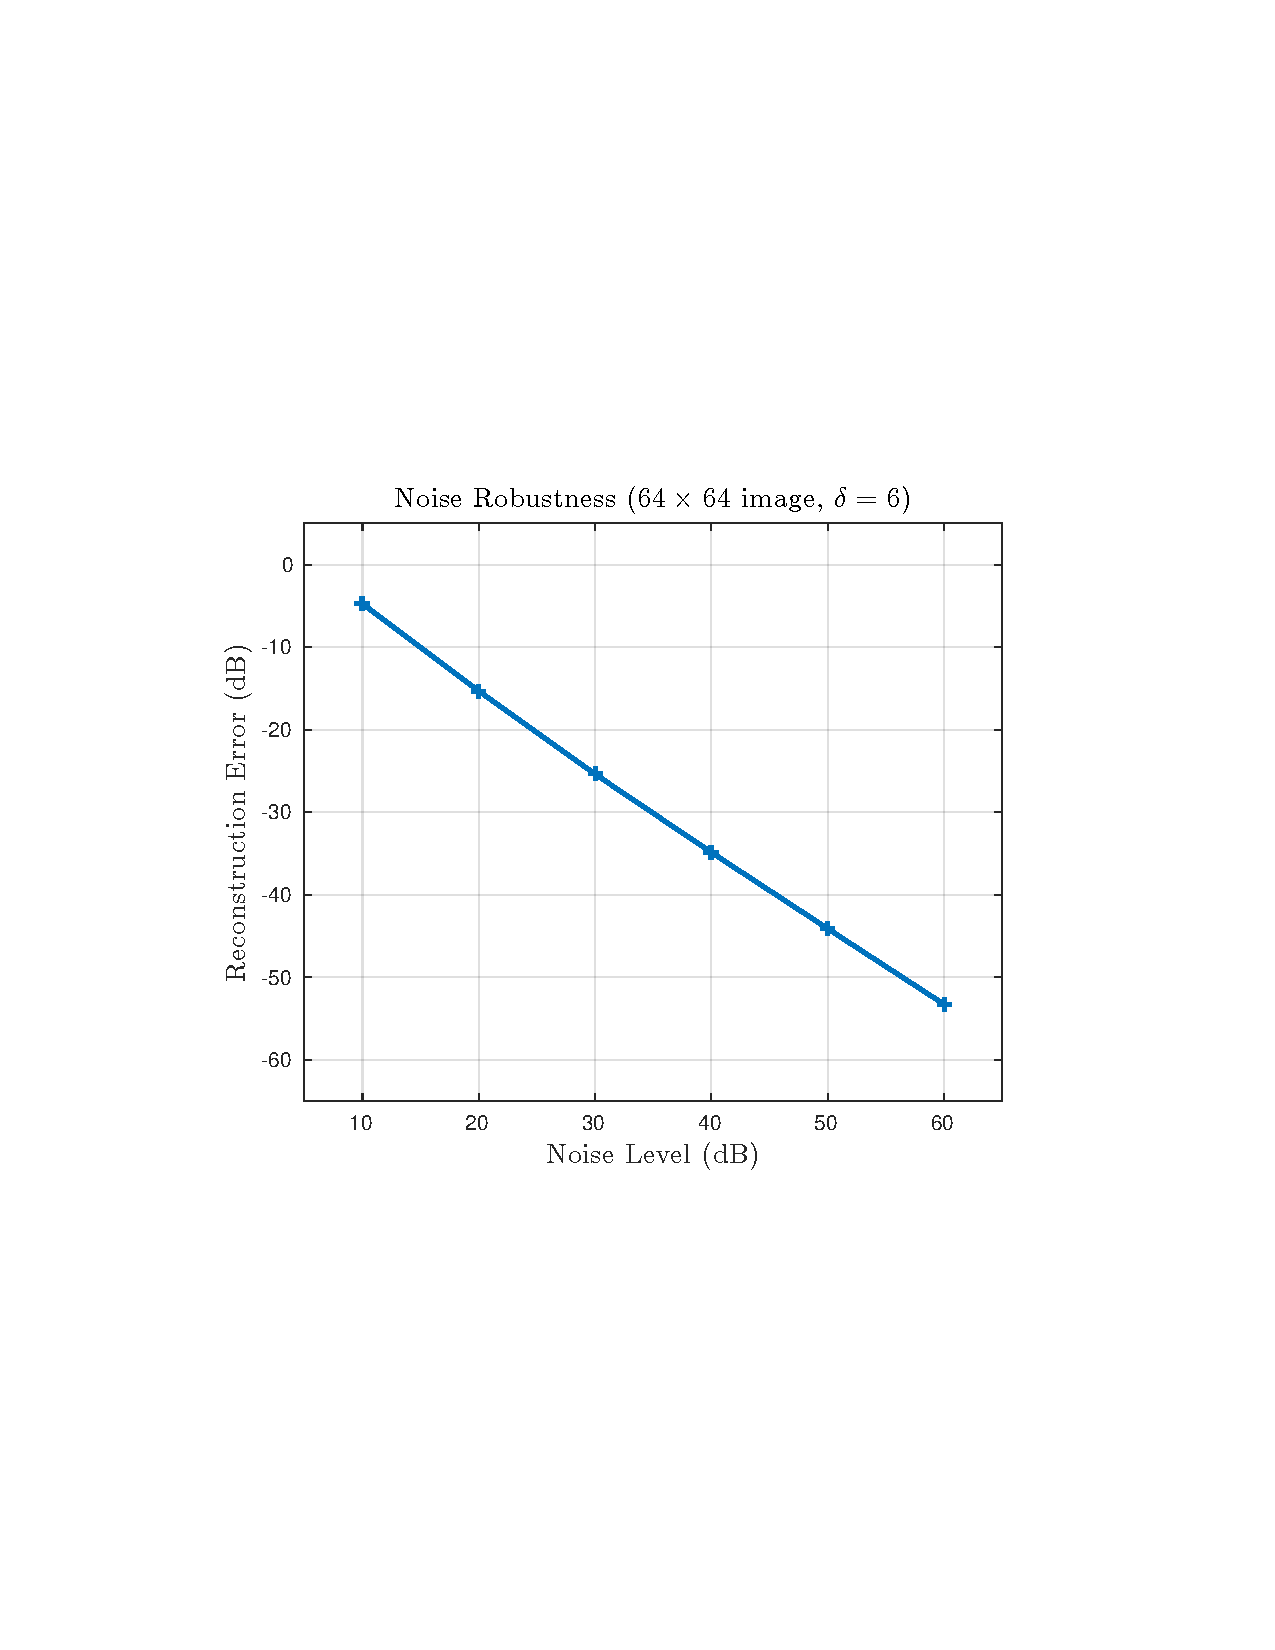
\includegraphics[clip=true, trim = 1.10in 3.15in 0.75in 3in,scale=0.55]{2d_figs/noise}
        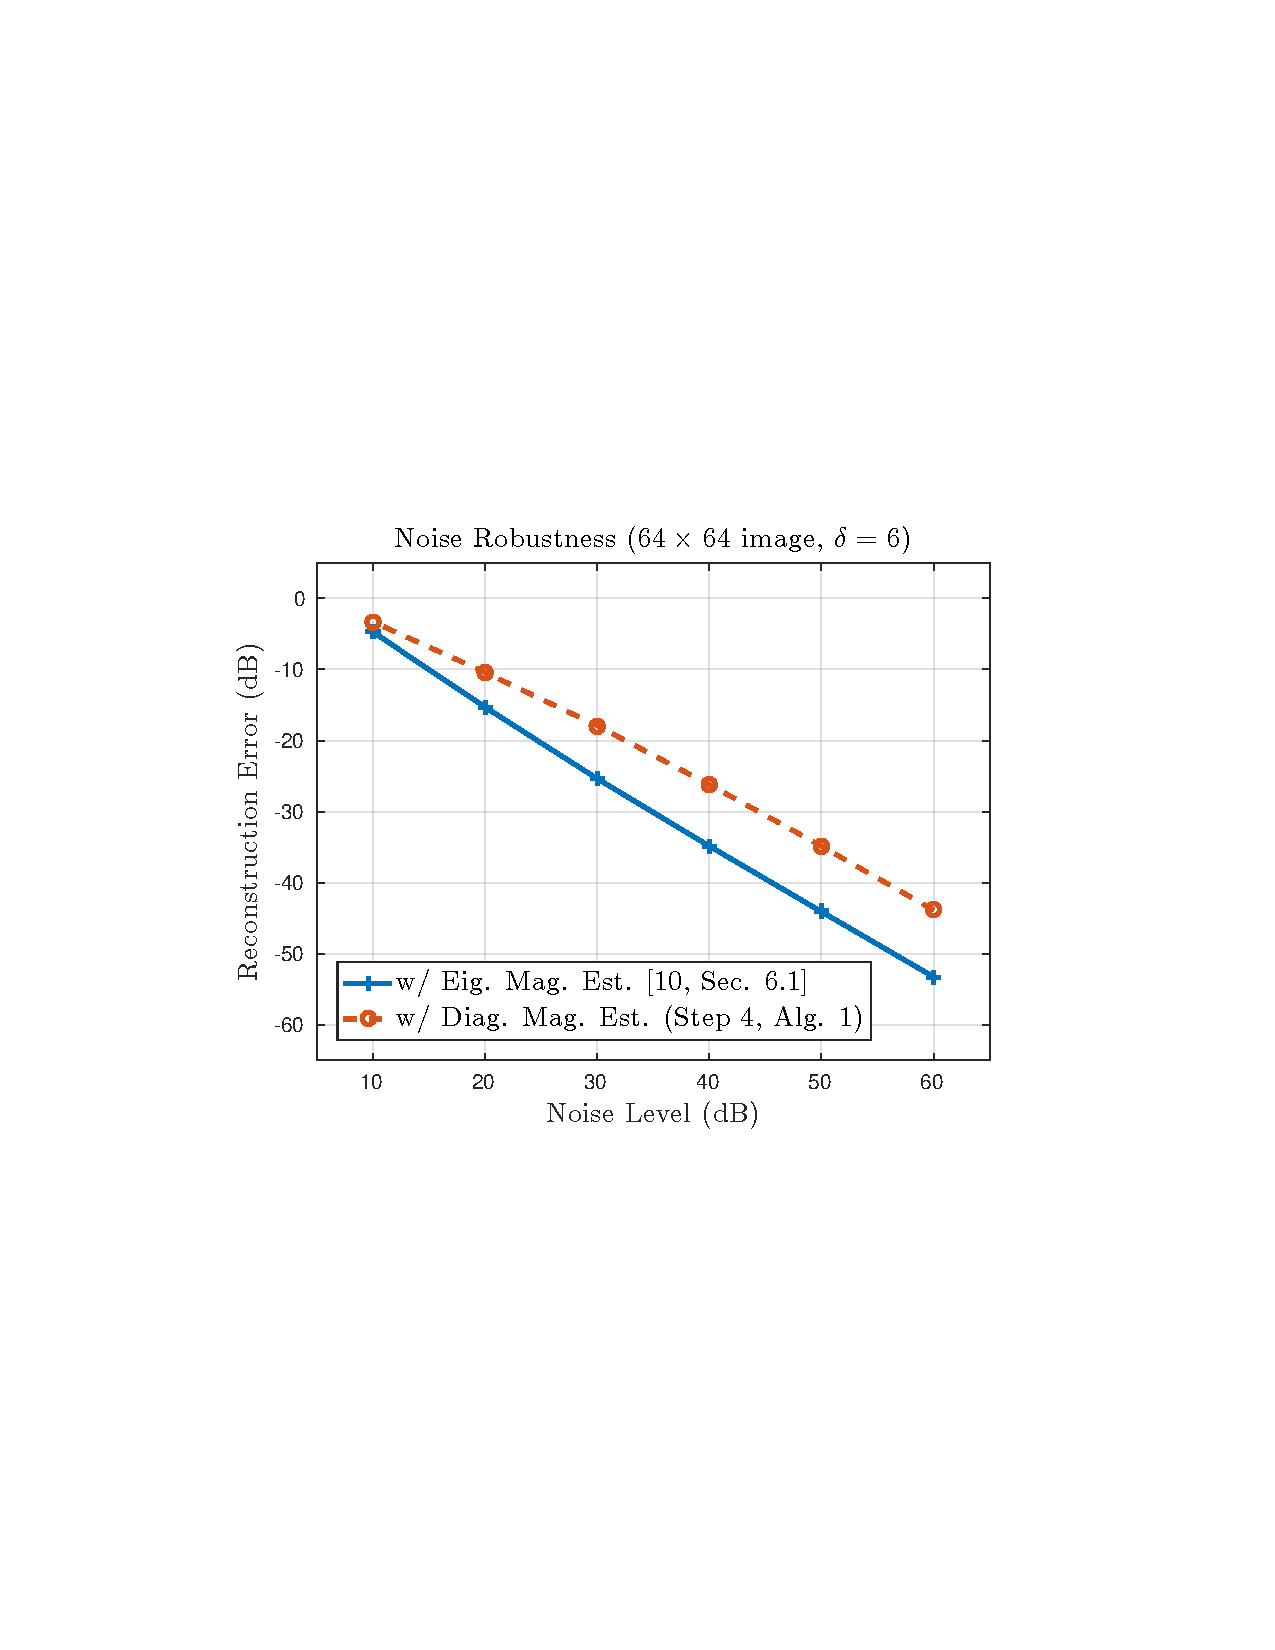
\includegraphics[clip=true, trim = 1.10in 3.25in 0.75in 3in,scale=0.575]{2d_figs/noise_alt}
        \caption{Noise Robustness of the Proposed Method}
        \label{fig:noise}
    \end{subfigure} 
    \vspace{0.05in}
    \caption{Evaluating the Efficiency and Robustness of the Proposed Two Dimensional Phase
    Retrieval Algorithm.}
    \label{fig:perf}
\end{figure}
%
